\tikzset{every picture/.style={line width=0.75pt}} %set default line width to 0.75pt        

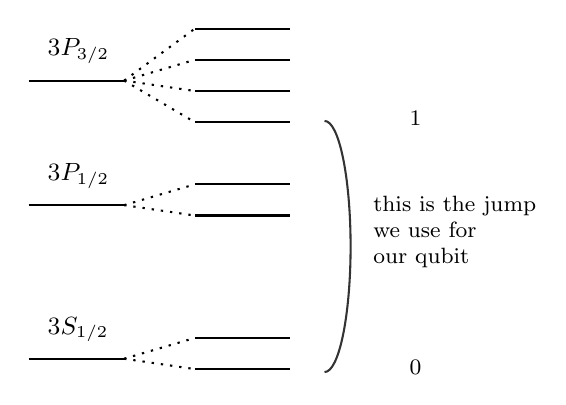
\begin{tikzpicture}[x=0.75pt,y=0.75pt,yscale=-1,xscale=1]
%uncomment if require: \path (0,190); %set diagram left start at 0, and has height of 190

%Straight Lines [id:da34059204718825886] 
\draw    (10,35) -- (25.97,35) -- (55.97,35) ;
%Straight Lines [id:da7025516674321846] 
\draw [line width=0.75]    (90,10) -- (105.97,10) -- (135.97,10) ;
%Straight Lines [id:da6658267546162004] 
\draw [line width=0.75]    (90,25) -- (105.97,25) -- (135.97,25) ;
%Straight Lines [id:da4714600148745056] 
\draw [line width=0.75]    (90,40) -- (105.97,40) -- (135.97,40) ;
%Straight Lines [id:da16901485927223803] 
\draw [line width=0.75]    (90,55) -- (105.97,55) -- (135.97,55) ;
%Straight Lines [id:da1939490218190003] 
\draw  [dash pattern={on 0.84pt off 2.51pt}]  (55.97,35) -- (90,10) ;
%Straight Lines [id:da5816163902648138] 
\draw  [dash pattern={on 0.84pt off 2.51pt}]  (55.97,35) -- (90,25) ;
%Straight Lines [id:da610618410737474] 
\draw  [dash pattern={on 0.84pt off 2.51pt}]  (55.97,35) -- (90,55) ;
%Straight Lines [id:da9192678870004782] 
\draw  [dash pattern={on 0.84pt off 2.51pt}]  (55.97,35) -- (90,40) ;
%Straight Lines [id:da9929664262930785] 
\draw    (10,95) -- (25.97,95) -- (55.97,95) ;
%Straight Lines [id:da5065393969849171] 
\draw [line width=0.75]    (90,85) -- (105.97,85) -- (135.97,85) ;
%Straight Lines [id:da5118777096116628] 
\draw [line width=0.75]    (90,100) -- (105.97,100) -- (135.97,100) ;
%Straight Lines [id:da5444849394573406] 
\draw  [dash pattern={on 0.84pt off 2.51pt}]  (55.97,95) -- (90,85) ;
%Straight Lines [id:da7828314169133617] 
\draw  [dash pattern={on 0.84pt off 2.51pt}]  (55.97,95) -- (90,100) ;
%Straight Lines [id:da31797955021255253] 
\draw    (10,169) -- (25.97,169) -- (55.97,169) ;
%Straight Lines [id:da7584898264764725] 
\draw [line width=0.75]    (90,159) -- (105.97,159) -- (135.97,159) ;
%Straight Lines [id:da14741105203655902] 
\draw [line width=0.75]    (90,174) -- (105.97,174) -- (135.97,174) ;
%Straight Lines [id:da2103499876371232] 
\draw  [dash pattern={on 0.84pt off 2.51pt}]  (55.97,169) -- (90,159) ;
%Straight Lines [id:da47885891493979593] 
\draw  [dash pattern={on 0.84pt off 2.51pt}]  (55.97,169) -- (90,174) ;
%Shape: Arc [id:dp22001354960228459] 
\draw  [draw opacity=0] (152.54,54.43) .. controls (152.54,54.43) and (152.54,54.43) .. (152.54,54.43) .. controls (159.46,54.43) and (165.08,81.51) .. (165.08,114.93) .. controls (165.08,148.34) and (159.46,175.43) .. (152.54,175.43) -- (152.54,114.93) -- cycle ; \draw [color={rgb, 255:red, 51; green, 51; blue, 51 }  ,draw opacity=1 ]   (152.54,54.43) .. controls (159.46,54.43) and (165.08,81.51) .. (165.08,114.93) .. controls (165.08,148.34) and (159.46,175.43) .. (152.54,175.43) ;  

% Text Node
\draw (17.67,13.4) node [anchor=north west][inner sep=0.75pt]  [font=\small]  {$3P_{3/2}$};
% Text Node
\draw (17.67,73.4) node [anchor=north west][inner sep=0.75pt]  [font=\small]  {$3P_{1/2}$};
% Text Node
\draw (17.67,147.4) node [anchor=north west][inner sep=0.75pt]  [font=\small]  {$3S_{1/2}$};
% Text Node
\draw (174.5,89) node [anchor=north west][inner sep=0.75pt]  [font=\footnotesize] [align=left] {this is the jump\\we use for\\our qubit};
% Text Node
\draw (192,48.4) node [anchor=north west][inner sep=0.75pt]  [font=\footnotesize]  {$\ket{1}$};
% Text Node
\draw (192,168.4) node [anchor=north west][inner sep=0.75pt]  [font=\footnotesize]  {$\ket{0}$};


\end{tikzpicture}
